% ---------------------------------------------------------------
% Chapter 2: Related Work
% ---------------------------------------------------------------
\chapter{Related Work} \label{cap:related-work}

Two bodies of work bear on this project: GCC's established mechanisms for synthesizing
hardware-absent operations, applied in the embedded domain for decades; and pedagogical tools for
instruction-set-level computing education.

\section{Instruction Synthesis in Compiler Backends}

GCC has long supported targets whose processors lack hardware instructions for certain operations. The
canonical example is soft-float: on a target without a floating-point unit, the compiler replaces every
floating-point operation by a call to a library routine that implements IEEE~754 arithmetic with
integer instructions, with no change required from the programmer \cite{gcc-internals}. Two properties
of that substitution matter here, and both reappear in this work. The first is that the replacement is
a body of carefully validated software arithmetic rather than an incidental expansion: the Berkeley
SoftFloat package \cite{softfloat} is the reference implementation of that kind, and is the arithmetic
model inside the Spike simulator against which this work validates its own output. The second is that
the substitution is an ABI contract rather than a private decision of one compiler. The Arm run-time
ABI \cite{arm-rtabi} names each helper routine and fixes its calling convention, so that soft-float
objects produced by different compilers interoperate; GCC documents the equivalent set for its own
targets as part of libgcc \cite{gcc-internals}, where the same mechanism extends to integer operations,
with routines such as \texttt{\_\_mulsi3} and \texttt{\_\_ashlsi3} existing precisely because some
targets have neither a multiplier nor a multi-bit shift.

Those integer cases are the closest existing precedent for this work. The MSP430 has no multi-bit shift
instruction: a shift by more than one position is either a repeated single-bit operation or a call to
one of the runtime helpers the MSP430 embedded ABI defines for the purpose, among them
\texttt{\_\_mspabi\_slli\_n}, \texttt{\_\_mspabi\_srli\_n} and their long and arithmetic variants
\cite{msp430-eabi,msp430-ug}. The AVR is more restricted still. Its shift and rotate instructions move
exactly one bit \cite{avr-isa}, so GCC's AVR backend emits a straight-line run of \texttt{lsl} or
\texttt{lsr} for a small constant count and a counted loop for a variable one --- the same two
constructions this work derives for rvsc1 in Section~\ref{sec:sc1-sll}, reached independently from the
same constraint. Hardware multiplication is likewise present only on the enhanced AVR cores; on the
classic and reduced-tiny devices \texttt{\_\_mulqi3} and \texttt{\_\_mulhi3} are shift-and-add routines
in libgcc \cite{avr-isa}. \citeonline{hauser2020} quantify what such substitutions cost on embedded
RISC-V targets, showing that backend choices have a measurable impact on code size.

In all these cases the programmer writes standard C and the compiler silently emits the replacement
sequence, at the cost of additional instructions and a correspondingly larger binary. What
distinguishes the present work is the proportion of the instruction set involved. A soft-float or
multiplier-less target is missing a category of operations; the sc0 and sc1 targets are missing nearly
everything, and must synthesize shifts, exclusive or, ordered comparisons, all conditional branches
other than \texttt{beq}, every sub-word load and store, and --- on sc0 --- the loading of a large
constant, out of eight or ten remaining instructions.

\section{Pedagogical Instruction-Set Tools}

A distinct body of work provides tools for computer architecture education at the assembly level. Venus
\cite{venus}, RARS \cite{rars}, and MARS \cite{mars} are simulators that accept programs written
directly in assembly and execute them step by step. None of them performs C compilation; the programmer
works at the assembly level from the outset.

BRISC-V \cite{brisc-v} provides an open-source parameterised RISC-V processor family for computer
architecture education together with a standard GCC toolchain. The toolchain targets the full RV32I
instruction set, with no mechanism to restrict the compiler to a hardware-defined subset.

This work sits at the intersection of the two lines: it brings the instruction synthesis approach
from the embedded compiler domain, applied to a far smaller instruction subset,
into the pedagogical setting of the Hennessy-Patterson processor \cite{patterson2020},
enabling students to write C programs that run correctly on a processor with a deliberately minimal
instruction set --- one they built themselves, which is what the assembly-level simulators and the
full-ISA toolchains each leave out.


% ---------------------------------------------------------------
% Chapter 3: Conceptual Background
% ---------------------------------------------------------------
\chapter{Conceptual Background} \label{cap:background}

\section{RISC-V}

RISC-V is an open, royalty-free instruction set architecture belonging to the Reduced Instruction Set
Computer (RISC) family \cite{riscv-spec}. RISC architectures favour a small number of simple,
orthogonal instructions over a large set of complex ones: all computation operates on registers, memory
is accessed exclusively through explicit load and store instructions, and instructions are fixed-width,
which keeps decoding logic simple and regular. The name RISC-V denotes the fifth major RISC ISA
developed at UC Berkeley. Unlike earlier RISC designs, RISC-V is fully open: anyone may implement it
without a license. The ISA is organized as a small mandatory base plus a set of optional standard
extensions, so implementors include only the features their application requires.

The base integer ISA has 32 general-purpose registers, x0--x31. x0 is hardwired to the constant zero
and reads as zero regardless of writes. The remaining registers are general-purpose; the ABI assigns
mnemonic names: a0--a7 for function arguments and return values, ra for the return address, sp for the
stack pointer, t0--t6 for caller-saved temporaries, and s0--s11 for callee-saved registers
\cite{riscv-spec}.

The RV32I base ISA contains approximately 40 instructions organised into functional groups: integer
arithmetic and logic (ADD, SUB, AND, OR, XOR, SLL, SRL, SRA and their immediate-operand forms ADDI,
ANDI, ORI, XORI, SLLI, SRLI, SRAI); loads and stores (LW, LH, LB and unsigned halfword/byte variants
LHU, LBU; SW, SH, SB); conditional branches (BEQ, BNE, BLT, BGE, BLTU, BGEU); jumps (JAL and JALR);
upper-immediate instructions (LUI and AUIPC); and environment/system instructions (ECALL, EBREAK,
FENCE) \cite{riscv-spec}.

Beyond the base, RISC-V defines several standard extensions. The M extension adds integer multiply and
divide (MUL, MULH, DIV, REM and variants). The A extension provides atomic memory operations
(load-reserved/store-conditional pairs LR/SC and a family of AMO instructions). The F and D extensions
add single- and double-precision IEEE~754 floating-point.

\section{Single-Cycle Processor Architecture}

A single-cycle processor completes every instruction in exactly one clock cycle. The datapath consists
of five principal components wired in sequence: an instruction memory that outputs the instruction at
the current program counter (PC), a register file with two read ports and one write port; an arithmetic
logic unit (ALU) that performs the operation selected by the control unit, a data memory for load and
store operations, and a set of multiplexers that route operands and results under control of the
control signals derived from the instruction opcode \cite{patterson2020}.
Figure~\ref{fig:datapath} shows these components and their interconnection for the eight-instruction
subset this work targets.

The control unit decodes the instruction's opcode field and drives the multiplexer select lines and the
register file write-enable. For a given instruction set, each instruction class has a fixed set of
control signals; the datapath itself does not change between instructions, only the routing of values
through the multiplexers changes. This regularity is what makes it tractable to add support for a new
instruction: each addition requires extending the decode logic and, where necessary, adding a new
datapath path or multiplexer input.

The critical path determines the maximum clock frequency. Because every instruction must complete
within one cycle, the clock period is set by the slowest instruction. For an RV32I processor the
critical path typically runs through instruction memory, the register file read ports, the ALU, data
memory (for \texttt{lw}), and the register file write port.

\section{Hennessy-Patterson Educational Processor}

\textit{Computer Organization and Design: RISC-V Edition} \cite{patterson2020} uses a series of
progressively more capable processor implementations to teach the relationship between instruction sets
and hardware. Chapter 4.4, titled \textit{A Simple Implementation Scheme}, introduces a single-cycle
datapath that supports only eight instructions: \texttt{lw}, \texttt{sw}, \texttt{beq}, \texttt{add},
\texttt{addi}, \texttt{sub}, \texttt{and}, and \texttt{or}. This restriction is deliberate: with only
eight instructions, the complete datapath and control unit fit on a single diagram and can be fully
understood and implemented within a single lab exercise.

The datapath for this subset is purpose-built. There is an ALU path for R-type arithmetic
(\texttt{add}, \texttt{sub}, \texttt{and}, \texttt{or}) and I-type arithmetic (\texttt{addi}), a
memory path for \texttt{lw} and \texttt{sw}; and a branch comparator for \texttt{beq}. The processor
has no hardware for PC-relative address computation (no AUIPC path), no mechanism to load a 20-bit
upper immediate into a register (no LUI path), and no register-to-PC write path that also captures
the return address (no JALR path). Executing any instruction outside the supported set produces
undefined results.

% Single-cycle datapath with control unit for the Hennessy-Patterson
% eight-instruction subset.
%
% This is the book's own Figure 4.21, reproduced as an image rather than
% redrawn, so that a reader holding the book sees exactly the diagram the
% course works from.  The credit line below the figure is mandatory: the
% illustration is the publisher's, not this work's.  The image file lives
% beside this .tex (and a second copy under ../figures/ feeds the Typst
% edition of the document).
\begin{figure}[htb]
\centering
\caption{The simple single-cycle datapath with the control unit, for the
         eight-instruction subset (\texttt{lw}, \texttt{sw}, \texttt{beq},
         \texttt{add}, \texttt{addi}, \texttt{sub}, \texttt{and}, \texttt{or})}
\label{fig:datapath}
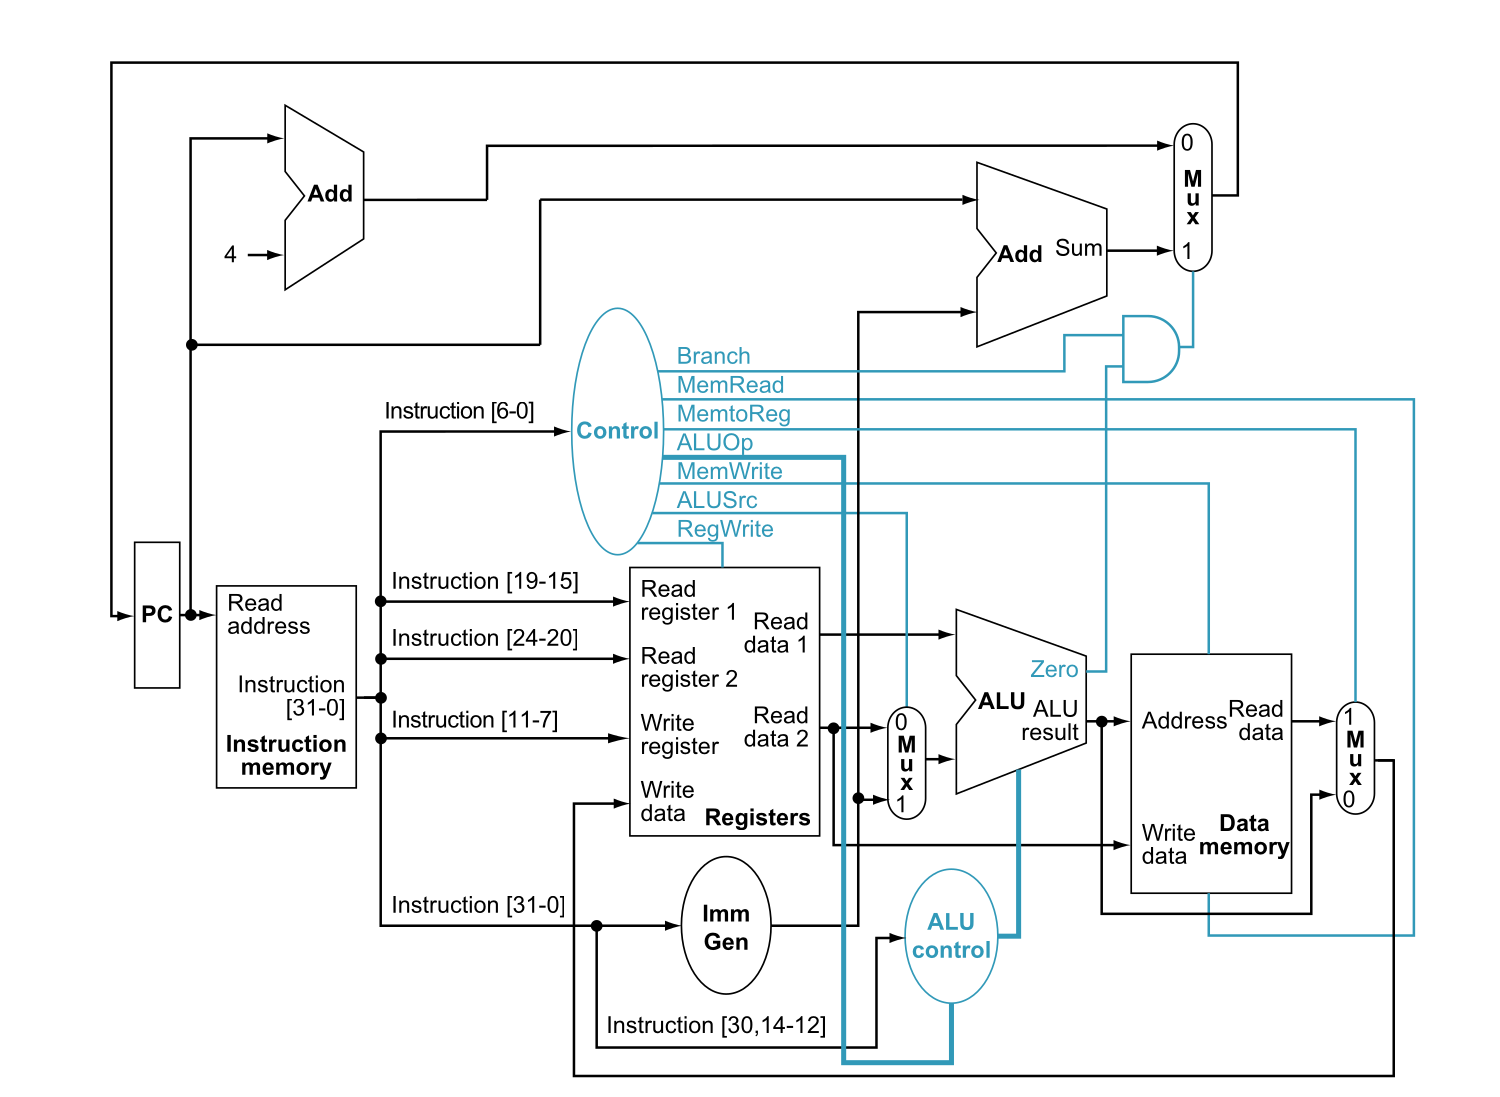
\includegraphics[width=\textwidth]{hannersy-patterson-implementation-fig4-21.png}
\fonte[Source]{Figure 4.21 of \citeonline{patterson2020} --- David A. Patterson
  and John L. Hennessy, \emph{Computer Organization and Design: RISC-V
  Edition}, 2nd ed., Morgan Kaufmann (an imprint of Elsevier), 2020.
  Reproduced here for academic purposes; copyright in the original
  illustration remains with the authors and the publisher.}
\nota[Note]{Black lines carry values and blue lines carry control signals.
  The subset has no upper-immediate path into the register file
  (\texttt{lui}), no \mbox{PC~+~4} write-back into the register file
  (\texttt{jal}, \texttt{jalr}), no register~$\rightarrow$~PC path
  (\texttt{jalr}) and no path from the \mbox{PC~+~immediate} adder into the
  register file, which only steers the PC multiplexer (\texttt{auipc}); each
  of those absences is the hardware reason for a synthesis derived in
  Section~\ref{sec:sc1-synthesis}.}
\end{figure}


The two absences that matter most for a compiler are visible in the figure as multiplexer inputs that
were never built. Without an upper-immediate input to the write-back multiplexer there is no single
instruction that places a large constant in a register, and without a PC-to-register path there is no
instruction that records a return address, which is what makes function calls impossible on rvsc0
(Section~\ref{sec:sc0-no-calls}). Every other restriction the subset imposes is an absent decode case
rather than an absent wire: the ALU and the branch comparator are already there, so \texttt{xor}, the
shifts and the ordered branches can be rebuilt out of the operations the datapath does route.

\section{C Calling Convention and ABI}

An Application Binary Interface (ABI) is the binary-level contract that allows separately compiled
translation units to interoperate. It specifies which registers hold function arguments, which the
caller must preserve across a call, which the callee must preserve, how the stack is laid out, and how
values are returned. Code compiled by different compilers for the same ABI can be linked and executed
together.

The RISC-V integer ABI partitions the 32 registers into four groups \cite{riscv-psabi}. Argument and
return-value registers (a0--a7, i.e.\ x10--x17) pass the first eight integer arguments to a function
and carry the return value back in a0 (and a1 for 64-bit values on RV32). Caller-saved temporaries
(t0--t6, i.e.\ x5--x7 and x28--x31) may be freely overwritten by any callee; the caller must save
them if their values are needed after a call. Callee-saved registers (s0--s11, i.e.\ x8--x9 and
x18--x27) must be preserved across calls; a callee that uses them must save and restore them.
Special-purpose registers are: ra (x1) the return address, sp (x2) the stack pointer, gp (x3) the
global pointer, and tp (x4) the thread pointer.

\begin{table}[htb]
\centering
\caption{RISC-V integer register conventions \cite{riscv-psabi}}
\label{tab:riscv-registers}
\begin{tabular}{llll}
\toprule
\textbf{Register} & \textbf{ABI name} & \textbf{Role} & \textbf{Saved by} \\
\midrule
x0        & zero    & Hardwired zero       & --- \\
x1        & ra      & Return address       & Caller \\
x2        & sp      & Stack pointer        & Callee \\
x3        & gp      & Global pointer       & --- \\
x4        & tp      & Thread pointer       & --- \\
x5--x7    & t0--t2  & Temporaries          & Caller \\
x8--x9    & s0--s1  & Saved registers      & Callee \\
x10--x11  & a0--a1  & Args / return value  & Caller \\
x12--x17  & a2--a7  & Arguments            & Caller \\
x18--x27  & s2--s11 & Saved registers      & Callee \\
x28--x31  & t3--t6  & Temporaries          & Caller \\
\bottomrule
\end{tabular}
\end{table}

The RISC-V stack grows downward. A typical stack frame contains, from high to low address: incoming
arguments that did not fit in a0--a7, the saved return address, saved callee-saved registers, and local
variables. The call sequence is: the caller loads arguments into a0--a7 (and pushes any extras onto
the stack), then executes \texttt{jal ra, target} to jump to the callee and record the return address
in ra. The callee saves ra and any s registers it uses, executes its body, places the result in a0,
restores saved registers, and returns with \texttt{jalr x0, 0(ra)} (the \texttt{ret}
pseudo-instruction). The stack pointer must be 16-byte aligned at every function entry and exit
\cite{riscv-psabi}.

GCC emits ELF (Executable and Linkable Format) object files. The principal sections are \texttt{.text}
(machine code), \texttt{.rodata} (read-only constants and string literals), \texttt{.data} (initialized
global variables), and \texttt{.bss} (zero-initialized global variables). Relocation entries in the
object file record every reference to a symbol whose address is not yet known; the linker fills these
in when it combines object files. A linker script controls the memory layout: it assigns each section
to an address range that matches the target processor's address map \cite{riscv-psabi}.

\section{GCC Compiler Architecture}

The GNU Compiler Collection (GCC) is a portable, multi-language, multi-target compiler and the
dominant toolchain for embedded and systems software \cite{gcc-internals}. It translates C (and other
languages) to machine code through a sequence of intermediate representations that progressively lower
the abstraction level.

The compilation pipeline proceeds as follows \cite{gcc-internals}, and is summarised in
Figure~\ref{fig:pipeline}. The language frontend parses source
code and produces an abstract syntax tree (AST). The AST is lowered to GIMPLE, a high-level,
language-independent, statement-level intermediate representation in static single-assignment (SSA)
form. The middle-end applies target-independent optimisations to GIMPLE (constant folding, inlining,
loop transformations, and others). GIMPLE is then lowered to RTL (Register Transfer Language), a
low-level IR that models instructions as operations on pseudo-registers and memory. The backend
operates on RTL to produce assembly.

The backend performs three main tasks \cite{gcc-internals}. Instruction selection pattern-matches RTL
expressions against the target's machine description to select real instructions. Register allocation
assigns the potentially unbounded set of pseudo-registers to the finite set of physical registers,
inserting spill code where necessary. Instruction scheduling reorders instructions to hide pipeline
latency and improve throughput; it is irrelevant for single-cycle processors, which have no pipeline
and therefore no data hazards.

The core of a GCC backend is the machine description file (\texttt{.md}), which declaratively
specifies the target's instruction set and expansion rules \cite{gcc-internals}. It contains two
primary construct types:

\begin{itemize}
  \item \texttt{define\_insn}: specifies a named RTL pattern, an assembly output template, and a
        predicate condition string that tests target capabilities. When the condition evaluates to
        false, the pattern is invisible to the instruction selector and will never be emitted.
  \item \texttt{define\_expand}: specifies a named operation that expands into an arbitrary sequence
        of RTL insns when the compiler needs to generate that operation. The expansion body may call
        \texttt{DONE} to signal that it has produced the complete implementation, preventing any
        fallthrough to a \texttt{define\_insn}. Expansions are the mechanism used to synthesize
        complex operations from simpler ones.
\end{itemize}

Code iterators (such as \texttt{any\_shift}) allow a single \texttt{define\_expand} to cover multiple
related operations (ASHIFT, LSHIFTRT, ASHIFTRT) in one body, with runtime-constant guards like
\texttt{(<CODE>) == ASHIFT} selecting the appropriate synthesis path.

% GCC compilation pipeline, marking the point where this work's synthesis
% happens (the RTL expansion pass, where `define_expand` bodies run).
%
% TikZ port of figures/pipeline.typ.  Conventions:
%   - solid boxes / arrows : the representations and the passes between them
%   - dashed grey boxes    : machine-description constructs acting at that step
\begin{figure}[htb]
\centering
\begin{SingleSpace}
\begin{tikzpicture}[
  x=0.74cm, y=0.74cm,
  font=\sffamily\fontsize{7}{8}\selectfont,
  stage/.style={draw, fill=black!4, inner sep=0pt, align=center,
                line width=0.5pt},
  flow/.style={-{Straight Barb[scale=0.55]}, line width=0.5pt},
  note/.style={draw=black!45, dashed, line width=0.4pt},
  notetext/.style={anchor=north west, text=black!55, align=left,
                   font=\sffamily\fontsize{5.5}{6.6}\selectfont},
  passlbl/.style={anchor=east, align=right,
                  font=\sffamily\fontsize{5.5}{6.6}\selectfont},
  bracket/.style={draw=black!50, line width=0.5pt},
]

\def\bxa{2.2}
\def\bxb{6.4}
\def\ax{4.3}

\newcommand{\Stage}[2]{%
  \path[stage] (\bxa,{#1-0.45}) rectangle (\bxb,{#1+0.45});
  \node at ({(\bxa+\bxb)/2},#1) {#2};}
% Vertical arrow between two stages, with the pass name to its left.
\newcommand{\Step}[3]{%
  \draw[flow] (\ax,{#1-0.45}) -- (\ax,{#2+0.45});
  \node[passlbl] at ({\ax-0.25},{(#1+#2)/2}) {#3};}
% Dashed note box on the right, with a pointer into the flow.
\newcommand{\Note}[4]{%
  \path[note] (10.2,#1) rectangle (18.1,#2);
  \node[notetext] at (10.4,{#1-0.2}) {#4};
  \draw[note, -{Straight Barb[scale=0.5]}] (10.2,#3) -- ({\ax+0.15},#3);}
% Phase bracket down the left-hand side.
\newcommand{\Phase}[3]{%
  \draw[bracket] (-0.5,#1) -- (-0.5,#2);
  \draw[bracket] (-0.5,#1) -- (-0.3,#1);
  \draw[bracket] (-0.5,#2) -- (-0.3,#2);
  \node[rotate=-90, text=black!60,
        font=\sffamily\fontsize{5.5}{6.6}\selectfont]
    at (-0.85,{(#1+#2)/2}) {#3};}

% --- the representations -------------------------------------------------
\Stage{0}{C source}
\Stage{-1.9}{GENERIC (AST)}
\Stage{-3.9}{GIMPLE, SSA form}
\Stage{-6.3}{RTL, pseudo-registers}
\Stage{-8.4}{RTL, hard registers}
\Stage{-10.2}{assembly (\texttt{.s})}
\Stage{-12.0}{ELF object}

% --- the passes between them ---------------------------------------------
\Step{0}{-1.9}{parse}
\Step{-1.9}{-3.9}{gimplify,\\SSA construction}
\Step{-3.9}{-6.3}{\textbf{RTL expansion}}
\Step{-6.3}{-8.4}{combine, register\\allocation (IRA/LRA),\\post-reload splits}
\Step{-8.4}{-10.2}{final: output\\templates}
\Step{-10.2}{-12.0}{\texttt{as} (binutils)}

\node[anchor=west, text=black!60, align=left,
      font=\sffamily\fontsize{5.5}{6.6}\selectfont\itshape]
  at ({\bxb+0.3},-3.9) {target-independent\\optimisation passes};

% --- phase brackets -------------------------------------------------------
\Phase{0.5}{-4.4}{front end + middle end}
\Phase{-4.9}{-10.7}{back end (target dependent)}

% --- what the machine description contributes, and where ------------------
\path[note] (10.2,0.5) rectangle (18.1,-1.15);
\node[notetext] at (10.4,0.3) {%
  \texttt{rvscN.h} \texttt{CC1\_SPEC} injects \texttt{-mno-shift},
  \texttt{-mno-xor}, \dots\\
  which clear the \texttt{riscv.opt} flags \texttt{TARGET\_SHIFT},\\
  \texttt{TARGET\_XOR}, \dots\ tested by every condition below};
\draw[note, -{Straight Barb[scale=0.5]}] (13.4,-1.15) -- (13.4,-3.7);

\Note{-3.7}{-5.7}{-5.1}{%
  \texttt{define\_expand} --- \textbf{where the synthesis happens.}\\
  With \texttt{-mno-shift}, \texttt{ashlsi3} expands to a chain of
  \texttt{add}\\
  instructions and calls \texttt{DONE}, so the \texttt{sll} pattern is never\\
  reached: the operation ceases to exist as RTL.}
\Note{-6.5}{-8.0}{-7.35}{%
  \texttt{define\_insn\_and\_split} --- splits that must run\\
  after register allocation, such as replacing\\
  \texttt{andi rd,rs,0xff} by \texttt{li} + \texttt{and}.}
\Note{-8.5}{-10.0}{-9.3}{%
  \texttt{define\_insn} --- output templates. A pattern whose\\
  condition is false (\texttt{TARGET\_SHIFT} on rvsc1) is\\
  invisible to instruction selection.}

\end{tikzpicture}

\vspace{0.4em}
{\footnotesize\color{black!60}\raggedright
The RTL expansion pass is where the synthesis of this work happens: a
\texttt{define\_expand} guarded by a \texttt{-mno-} flag emits a replacement
sequence and calls \texttt{DONE}, so the absent instruction never enters RTL and
no later pass can reintroduce it.\par}

\end{SingleSpace}
\caption{GCC compilation pipeline and the machine-description construct acting
         at each step}
\label{fig:pipeline}
\end{figure}


The position of that expansion step in the pipeline determines what the rest of this work can and
cannot do. Because synthesis happens as GIMPLE is lowered to RTL, every subsequent pass, register
allocation included, sees only the replacement sequence and optimises it as ordinary code, which is
what makes the synthesis transparent. The same position also explains the loss discussed in
Section~\ref{sec:sc1-corner-cases}: once an \texttt{xor} has become an \texttt{and}, an \texttt{or} and
a \texttt{sub}, no later pass can recognise the algebraic identities of the operation it replaced, so
any identity worth exploiting must be folded inside the expansion body itself.

Target-specific command-line options are declared in a \texttt{.opt} file using GCC's
option-description syntax \cite{gcc-internals}. Each declaration generates a C preprocessor macro
that can be tested in \texttt{.md} condition strings and in C target-hook implementations. A
per-target header file defines \texttt{CC1\_SPEC}, a GCC macro evaluated when the driver invokes the
compiler proper (\texttt{cc1}). It contains conditional option-injection rules of the form ``if the
user did not explicitly pass a flag, inject its negation.'' This mechanism makes a target
self-configuring: users invoke the target-specific compiler without any manual flags, and the correct
behaviour is activated automatically.
